\label{section:running-example}
In this section we first provide an overview of our approach that does not include an equivalence minimization 
step. We then revisit the 
overview explaining where some aspects of minimization require special treatment.

\vspace{-0.5cm}
\subsubsection{Overview without Minimization.} Consider a control problem $\mathcal{E} = \langle \mathcal{M}, \Sigma_c, \varphi 
\rangle$ where $\mathcal{M}$ is a set of LTS. A monolithic approach to solving the 
problem (e.g., ~\cite{DIppolito2008}) composes all the LTSs in $\mathcal{M}$ and 
then computes a controller. 
Our approach starts with $\mathcal{M}$ and an empty set $\mathcal{C}$ which 
will store \textit{safe controllers} (we discuss them below).  We 
iteratively extract a subset $\mathcal{M}'$ of  $\mathcal{M}$ of size greater than 1, 
compose the LTSs in $\mathcal{M'}$, compute a safe controller for the composition (with 
a weaker property $\varphi'$ and a larger controllable alphabet -- we explain why below). 
and store it in $\mathcal{C}$. In addition, we reintroduce a controlled version of  
$\mathcal{M}'$ to $\mathcal{M}$, 
we refer to this LTS as an \textit{controlled subplant} (we explain these below).  

In each iteration, $\mathcal{C}$ increases by one and $\mathcal{M}$ decreases 
by at least one.
% \vb{Partial Synthesis no parece hacer esto. M se puede mantener del mismo tamaño al sacar uno sólo y reemplazarlo x la componente controlada. Eso no es malo de por sí (ej. puede servir para CM, por ejemplo) pero la idea de que M se reduce de tamaño es lo que no parece cierto.} 
The iteration ends if the subset $\mathcal{M}'$ (which is picked by a 
heuristic) is equal to $\mathcal{M}$, typically when $\mathcal{M}$'s size is 1 or 2. At this point we apply the standard monolithic 
approach for 
$\varphi$ to $\mathcal{M'}$. The controller built in this last step of the algorithm can be 
thought of as a 
\textit{live controller} in contrast to the safe controllers built before.

The \textit{solution} to the original control problem $\mathcal{E}$ is the composition of 
the safe controllers in $\mathcal{C}$ with the live controller computed after the 
iterations.

\paragraph{\textbf{Safe Controllers.}} We provide an intuition of what is referred to as 
safe controllers and why they are computed for a  property $\varphi'$ that is weaker than $\varphi$ and an 
expanded controllable alphabet. We do so by working through an example.

Consider the control problem $\langle \mathcal{M}, \Sigma_c, \varphi \rangle$  
depicted in Figure~\ref{fig:input-machines}. A monolithic synthesis approach would first 
compose the three LTSs in $\mathcal{M}$  and then compute a controller. The composition (see Fig.10 of the Appendix in the technical report submitted in Arxiv) has 23 states.



\begin{figure}
    \centering
    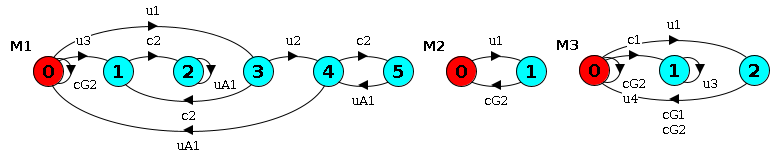
\includegraphics[width=.75\linewidth]{sections/example_img/imgs/fig_inputmachines.png}
    \caption{Modular plant for a control problem $\mathcal{E}$ with $ 
    \mathcal{M} = \{M_1, M_2, 
    M_3\}$,  GR(1) goal $\varphi = \always\eventually uA1 \implies
    \always \eventually cG1 \wedge \always \eventually cG2$ and  controllable alphabet 
    $\Sigma_c = \{cG1, cG2, c1, c2\}$.}
    \label{fig:input-machines}
\end{figure}


Consider a first iteration of our  algorithm in which a heuristic selects the subset 
$\mathcal{M'} = \{M_1, M_2\}$ and computes it  composition (see  Fig. 
\ref{fig:M1_M2}).


\begin{figure}[h!]
\centering
\begin{minipage}[b]{.47\textwidth}
  \centering
  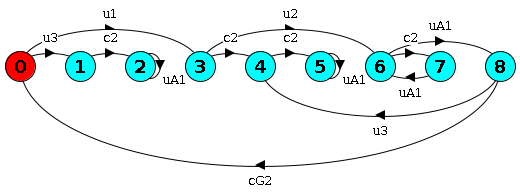
\includegraphics[width=.9\linewidth]{sections/example_img/imgs/fig_M1_M2.png}
    \caption{Parallel composition of subplant $\mathcal{M}' = \{M_1, M_2\} \subset 
    \mathcal{M}$, i.e., $M_1 \| M_2$.
    % \su{Asumo que M1 no va a tener un estado -1 y que u3 desde 0 y c2 desde 1 van a ir a un estado 4 donde se sólo se puede hacer c2 y se llega a un estado 5 donde se hace loop en uA1}
    }
    \label{fig:M1_M2}
\end{minipage}\hspace{0.03\textwidth}%
\noindent
\begin{minipage}[b]{.48\textwidth}
    \centering
    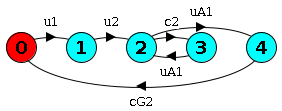
\includegraphics[width=.6\linewidth]{sections/example_img/imgs/fig_safecontroller.png}
    \caption{Safe Controller $(\M_1 \| M_2)_{\mbox{\textit{\scriptsize safe}}}$ for 
    subplant $M_1 \| M_2$, 
    $\varphi' =  \always\eventually 
    uA1 
    \implies \top \wedge \always\eventually cG2$, controllable events 
    $\Sigma_c \cup \{u3\}$, and $\mu = \emptyset$.% It is safe as it does not enforce $\varphi'$ but 
    %any controller that enforces $\varphi'$ is less or equally permissive.
    }
    \label{fig:safe-controller}
    
  % \centering
  % \includegraphics[width=.4\linewidth]{sections/example_img/fig3_M1||M2.png}
  % \caption{figure}{Another figure}
  % \label{fig:test2}
\end{minipage}
\end{figure}

We would like to  control $\mathcal{M}'$ to achieve $\varphi$. However, 
this is not possible as $\varphi$ refers to $cG1$ that is  not in the alphabet of the LTS in 
$\mathcal{M}'$. Thus, we weaken $\varphi$  by \textit{projecting} it to the alphabet of 
$\mathcal{M}'$:  $\varphi' = \always\eventually uA1 \implies \top 
\wedge \always\eventually cG2$ .% We discuss projection in Section~\ref{subsection:partial-synth}. \hg{Revisar si esto se mantiene.}
 
 Now we would like to control $\mathcal{M}'$ to achieve the weaker 
  $\varphi'$. Yet this is not 
  possible because a controller cannot prevent the occurrence of $u3$ in the initial state 
  of $\mathcal{M}'$. 
 But event $u3$ would never occur in the initial state of the plant $\mathcal{M}$ 
 because $M_3 \not\in \mathcal{M'}$ disallows it in its initial state!  Indeed, when 
 computing a controller for $\mathcal{M'}$ we must account for the fact that certain 
 aspects of the problem may be solvable when considering the rest of the plant. For this 
 we \textit{expand the controllable alphabet} to include all uncontrollable events shared 
 with LTS 
 in $\mathcal{M} \setminus \mathcal{M'}$ (i.e., $u3$).
  

  
  We now explain why we compute a \textit{safe} controller for the weaker formula $\varphi'$ 
  and the extended set of controllable events:   There may be controllers that can realize 
  $\varphi'$ in different ways (often called strategies). Some of these strategies may be 
  conflicting with restrictions imposed by LTS in $\mathcal{M} \setminus \mathcal{M'}$ 
  or parts of the goal lost in the projection of $\varphi$.  Ideally, we would compute a 
  controller that includes all such strategies, but this is impossible. Liveness goals such as 
  GR(1) do not allow maximally permissive controllers. Instead  of constructing a 
  controller that achieves $\varphi'$ we build one that avoids states in $\mathcal{M}'$ 
  that a controller that guarantees   $\varphi'$ may traverse. In other words, we build a 
  controller that stays in winning states of $\varphi'$. This is a safety property, and if 
  there is a controller, there is a maximally permissive one. 
  
  The safe (maximally permissive) controller for $\mathcal{M'}$, $\varphi$, and 
  $\Sigma_c \cup \{u3\}$, referred to as $(M_1 \| M_2)_{\mbox{\textit{\scriptsize 
  safe}}}$    is 
  shown in 
  Fig.\ref{fig:safe-controller} 
  and is added to $\mathcal{C}$.
  
  \paragraph{\textbf{Controlled Subplant.}} We now provide an intuition of what  
  controlled subplants are. Having computed a safe 
  controller   for $M_1 \| M_2$  for a weaker goal than $\varphi$ we must describe what 
  remains to be controlled. 
  
  A  naive approach would be to add to  $\mathcal{M}$ the controlled version of  
  $M_1 \|    M_2$, in other words $(M_1 \| M_2)_{\mbox{\textit{\scriptsize 
      safe}}} || (M_1 \| M_2)$. However, 
  the $(M_1 \| M_2)_{\mbox{\textit{\scriptsize 
    safe}}}$  was built assuming it controlled $u3$ when in fact it does not. Indeed, the 
    composition would not let the subplant $M_1 \|    M_2$ take a $u3$ transitions   
    from states 0 and 8. 
    
    To adequately model the behavior of the controlled subplant (see 
    Fig.\ref{fig:partial-controller})   
     we must re-introduce  
    $u3$ transitions to the safe controller. Specifically, we must add them to states 0 and 4 
    of the controller, these are the states the controller would be in if it were composed with 
    the subplant and the subplant were in states 0 or 8. Added transitions are sent to a 
    deadlock state because we know that from this point on, it is impossible to achieve 
    $\varphi'$ and thus  impossible to achieve  $\varphi$.  
    
    Indeed, the safe controller with the added transitions and deadlock state represent the 
    safe controller with the assumptions it makes on  when uncontrolled shared  events 
    should not happen. The deadlock state is in a sense abstracting states 1, 2, 4 and 5 of the 
    subplant $M_1 \| M_2$ of Fig.~\ref{fig:M1_M2} as bad states. 
    
  \begin{figure}[h!]
        \centering        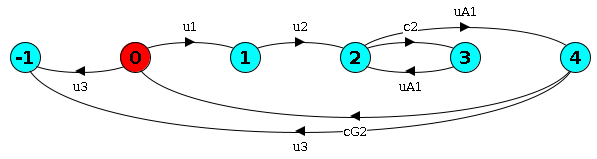
\includegraphics[width=.5\linewidth]{sections/example_img/imgs/fig_safeasmcontroller.png}
        \caption{Controlled Subplant $(M_1 || M_2)_{\mbox{\textit{\scriptsize 
          cont}}}$ 
        %for $\varphi' =  \always\eventually         uA1 \xrightarrow[]{} \text{true} \wedge 
        %\always\eventually g2$, and controllable         events $\Sigma_c \cup \{uS\}$. 
         built from the safe controller $(M_1 || M_2)_{\mbox{\textit{\scriptsize 
          safe}}}$ in
        Fig.~\ref{fig:safe-controller} by adding $u3$ transitions from state 0 and state 4 to a 
        deadlock state}	
        \label{fig:partial-controller}
    \end{figure}

    
  
  
    
  \paragraph{\textbf{After the First Iteration.}}
  At the end of the first iteration of our simplified algorithm we have: $\mathcal{M} = 
  \{M_3, (M_1 \| 
  M_2)_{\mbox{\textit{\scriptsize 
    cont}}}\}$   and $\mathcal{C} =\{ (M_1 \| M_2)_{\mbox{\textit{\scriptsize 
      safe}}}\}$.  As the subplants are required to be of size larger than 1, the only possible   
      $\mathcal{M'} \subseteq \mathcal{M}$ is actually $\mathcal{M}$. Here termination 
      of the iterations kicks in and the algorithm proceeds to build a 
  live controller using a monolithic approach for:  $\langle \{M_3, 
  (M_1 \| M_2)_{\mbox{\textit{\scriptsize 
    cont}}}\}, \Sigma_c, \varphi \rangle$. In other words, it builds the plant $M_3 \| 
    (M_1 
  \| M_2)_{\mbox{\textit{\scriptsize 
    cont}}}$ (see Fig.11 in Appendix of the technical report submitted in Arxiv), 
   computes a controller 
  $(M_3 \| (M_1 \| 
  M_2)_{\mbox{\textit{\scriptsize 
    cont}}})_{\mbox{\textit{\scriptsize 
      live}}}$ (see Fig.~\ref{fig:controllerIt1}) and returns the 
  solution $\mathcal{C} = \{(M_3 \| (M_1 \| 
  M_2)_{\mbox{\textit{\scriptsize 
    cont}}})_{\mbox{\textit{\scriptsize 
      live}}},$ $(M_1 \| M_2)_{\mbox{\textit{\scriptsize 
        safe}}}\}$. 
  
  
    
      
        \begin{figure}[h!]
              \centering
              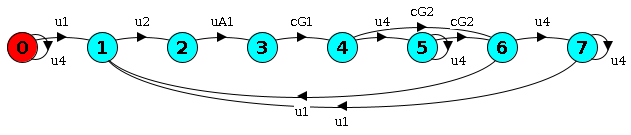
\includegraphics[width=.55\linewidth]{sections/example_img/imgs/fig_controllerIt1.png}
              \caption{Controller $(M_3 \| (M_1 \| 
                M_2)_{cont})_{live}$ for Fig.11. 
                }
              \label{fig:controllerIt1}
          \end{figure}
      
      
      
        
      
 Note that the largest LTS for which the compositional algorithm built a controller 
 was of size 14, whilst a monolithic approach applied to $M_1 \| M_2 
 \| M_3$ would have 
 had to analyse an LTS of size 22.


        
\subsubsection{Introducing Minimization.} The approach to synthesis presented formally in the next sections relies heavily on 
minimization to perform well: It minimizes the controlled subplants before adding them to $\mathcal{M}$.  The minimization procedure preserves the 
synthesis observational equivalence defined in~\cite{mohajerani_algorithm_2012}. We 
apply minimization, as does~\cite{mohajerani_algorithm_2012}, hiding events that are 
local to the controlled subplant (i.e., events that are not part of the alphabet of the remaining LTSs in 
$\mathcal{M}$). In Fig.~\ref{fig:abstraction} we depict the minimized 
version of $(M_1 \| 
M_2)_{\mbox{\textit{\scriptsize 
  cont}}}$ using local events $\Upsilon = \{u2, uA1, c2\}$. Note that minimization may introduce non-determinism that can be solved, as in~\cite{mohajerani_algorithm_2012} using relabeling.  

\begin{figure}[h!]
\centering
\begin{minipage}[b]{.45\textwidth}
  \centering
  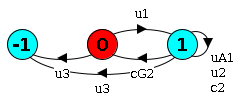
\includegraphics[width=.55\linewidth]{sections/example_img/imgs/fig_safeasmcontrollerreduced.png}
   \caption{$(M_1 \| 
    M_2)_{\mbox{\textit{\scriptsize 
      cont}}} / \! \!\sim_{\Upsilon}$, a minimized version of 
      $(M_1 \| 
         M_2)_{\mbox{\textit{\scriptsize 
           cont}}}$ with local events $\Upsilon = \{u2, uA1, c2\}$.}
    \label{fig:abstraction}
\end{minipage}\hspace{0.02\textwidth}%
\noindent
\begin{minipage}[b]{.5\textwidth}
    \centering
    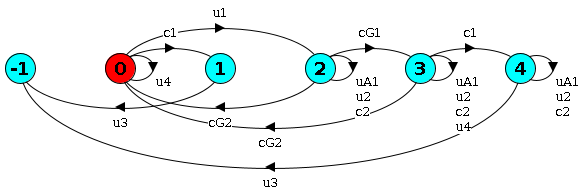
\includegraphics[width=1\linewidth]{sections/example_img/imgs/fig_reduced_M3.png}
    \caption{Plant $(M_1 || M_2)^{c} / \sim_{\Upsilon} || M_3$ to be controlled assuming 
    $\square \Diamond \  (\neg  u2  \wedge  \neg uA1 \wedge \neg c2)$)}
    \label{fig:compose_singleton}
\end{minipage}
\end{figure}

The approach proceeds by composing $(M_1 \| M_2)_{\mbox{\textit{\scriptsize 
  cont}}} / \!\!\sim_{\Upsilon}$ and 
$M_3$  (see Fig.\ref{fig:compose_singleton}) and 
attempts to build a controller for 
$\varphi$. 
However, such a controller does not exists as the trace $u1.uA1^\omega$ cannot be 
avoided. Yet such a trace is not possible in $(M_1 \| M_2 \| M_3)$ (see 
Fig.10 in Appendix of the technical report submitted in Arxiv).  This mismatch can be  traced back to the minimization procedure that introduces a 
looping transition labelled $uA1$ in state 1 in  $(M_1 \| 
M_2)_{\mbox{\textit{\scriptsize 
  cont}}} /\!\!\sim_{\Upsilon}$ which $(M_1 \| M_2)_{\mbox{\textit{\scriptsize 
  cont}}}$ does not have. Note that these loops are not a problem for compositional control for finite traces such as in~\cite{mohajerani_algorithm_2012}.




    Having introduced uncontrollable looping transitions, they must be kept track of  (we add them to a set $\mu$) and solve control problems in 
    future iterations that assume events in $\mu$  do not occur infinitely (i.e.,  $\always\eventually  \bigwedge_{l\in\mu} \neg l \implies  \varphi$). Although not a GR(1) formula, it can be solved using GR(1) synthesis.

The live controller for $(M_1 \| M_2)_{\mbox{\textit{\scriptsize 
  cont}}} / \sim_{\Upsilon} \| M_3$  and 
property  
$\always\eventually  \bigwedge_{l\in\mu} \neg l \implies \varphi$ is depicted 
on the 
left of Fig. 
\ref{fig:compositional_controller}. This live controller plus the safe 
controller in 
Fig.~\ref{fig:safe-controller} are a modular solution to 
$\mathcal{E}$. 

\begin{figure}[h!]
    \centering
    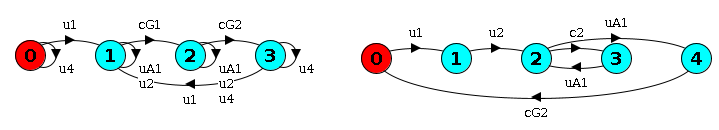
\includegraphics[width=.7\linewidth]{sections/example_img/imgs/fig_compositionalcontroller.png}
    \caption{Modular representation of a controller for the discrete event problem 
    $\mathcal{M} = \{M_1, M_2, M_3\}$ to be controlled to satisfy $\varphi = 
    \always\eventually uA1 \implies \always \eventually cG1 \wedge \always 
    \eventually cG2$ with controllable alphabet $\Sigma_c = \{cG1, cG2, c1, c2, c3\}$.
     Controller on the left is a solution to Fig.\ref{fig:compose_singleton}, controller on the 
     right is the safe controller from Fig.~\ref{fig:safe-controller}.} 
    \label{fig:compositional_controller}
\end{figure}


            
Note that using minimization, the largest LTS for which synthesis was computed for has 5 
states, while a monolithic approach would have computed a controller for a plant of 22 
states. This exemplifies how state explosion of the composed plant might be avoided using 
our compositional approach.


Subplant minimization can result in a non-deterministic monitor. To remove 
non-determinism we use a the same procedure as in ~\cite{mohajerani_algorithm_2012}.  
%where non-deterministic choices are renamed with fresh event names, a  function $\rho$ 
%is updated to keep track of these renamings, and $rho$-distinguishers are added to 
%$\mathcal{M}$ to ensure the final result can be mapped back to the original event 
%names. 
Due to space restrictions we do not discuss renaming in this paper, but our implementation and experimentation includes it. We refer the reader to 
~\cite{mohajerani_algorithm_2012} for more information. 

